\documentclass{article}
\usepackage{graphicx}
\usepackage{amsmath}
\usepackage{caption}
\usepackage{subcaption}
\usepackage{amssymb}
\usepackage{hyperref} % Include the hyperref package for URLs
\usepackage[backend=biber]{biblatex} % Include the biblatex package
\addbibresource{references.bib} % Specify the bibliography file

\begin{filecontents}{references.bib}
@misc{dealii,
    title = {deal.II Library: Matrix-Free Framework},
    howpublished = {\url{https://www.dealii.org/current/doxygen/deal.II/group__matrixfree.html}},
}

@misc{kronbichler2020,
    author = {Martin Kronbichler},
    title = {The State of Matrix-free Methods and HPC},
    howpublished = {\url{https://dealii.org/workshop-2020/slides-kronbichler-dealii-2020.pdf}},
    year = {2020}
}
\end{filecontents}


\title{Matrix Free ADR solver report}
\author{Luca Venerando Greco \and Alberto Guerrini \and Pierpaolo Marzo}
\date{April 2024}

\begin{document}

\maketitle

\section{Introduction}

Let us consider the following advection-diffusion-reaction (ADR) problem with mixed Dirichlet-Neumann boundary conditions:

\begin{equation}\label{eq:start_problem}
\begin{cases}
    -\nabla \cdot (\mu \nabla u) + \nabla \cdot (\boldsymbol{\beta} u) + \gamma u = f & \text{in } \Omega , \\
    u = g & \text{on } \Gamma_D \subset \partial \Omega , \\
    \nabla u \cdot n = h & \text{on } \Gamma_N = \partial \Omega \setminus \Gamma_D
\end{cases}
\end{equation}

\section{The Problem}
In this section we perform all the steps that are necessary to solve numerically the ADR problem in (\ref{eq:start_problem}).

A first consideration about the advective term must be done. If we take its divergence, it can be expanded as
\begin{equation}
    \nabla\cdot(\boldsymbol{\beta}u) = \boldsymbol{\beta}\cdot\nabla u + u\nabla\cdot\boldsymbol{\beta}
\end{equation}
where assuming an incompressible fluid, i.e. $\nabla\cdot\beta = 0$, the problem (\ref{eq:start_problem}) becomes
\begin{equation}\label{eq:adr_problem}
\begin{cases}
    -\nabla \cdot (\mu \nabla u) + \boldsymbol{\beta} \cdot \nabla u + \gamma u = f & \text{in } \Omega , \\
    u = g & \text{on } \Gamma_D \subset \partial \Omega , \\
    \nabla u \cdot n = h & \text{on } \Gamma_N = \partial \Omega \setminus \Gamma_D
\end{cases}
\end{equation}

\subsection{Weak formulation}
Let us start by introducing the function spaces
\begin{align}
    V &= \{v \in H^1(\Omega) \text{ such that } v = g \text{ on } \Gamma_D \} , \label{eq:2} \\
    V_0 &= \{v \in H^1(\Omega) \text{ such that } v = 0 \text{ on } \Gamma_D\}  \label{eq:3}
\end{align}
We write $u = u_0 + R_g$, where $u_0 \in V_0$ and $R_g \in V$ is an arbitrary lifting function such that $R_g = g$ on $\Gamma_D$.

Taking $v \in V_0$, multiplying it to \eqref{eq:adr_problem}, and integrating over $\Omega$, we get
\begin{equation}
    \int_{\Omega} -\nabla \cdot (\mu\nabla u) v \,d{\Omega} + \int_{\Omega} \boldsymbol{\beta} \cdot \nabla u v \,d{\Omega} + \int_{\Omega} \gamma u v \,d{\Omega} = \int_{\Omega} f v \,d{\Omega}
\end{equation}
Then integrating by parts, we have that:
\begin{equation}
    \int_{\Omega} -\nabla \cdot (\mu\nabla u) v \,d{\Omega} =  \int_{\Omega} \mu \nabla u \cdot \nabla v \,d{\Omega} - \int_{\partial\Omega} (\mu \nabla u \cdot n) v \,{\partial\Omega}
\end{equation}
And so we obtain, considering also that $\partial\Omega = \Gamma_d + \Gamma_n$ and that $v = 0$ on $\Gamma_d$:
\begin{equation}
   a(u,v)=F(v)
\end{equation}
where:
\begin{align}
    a(u,v) &= \int_{\Omega} \mu \nabla u \cdot \nabla v \,d{\Omega} + \int_{\Omega} \boldsymbol{\beta} \cdot \nabla u v \,d{\Omega} + \int_{\Omega} \gamma u v \,d{\Omega}\\
    F(v) &= \int_{\Omega} f v \,d{\Omega} + \int_{\Gamma_n} (\mu \nabla u \cdot n) v \,d{\Gamma_n}
\end{align}
Now, remembering that $u = u_0 + R_g$, we obtain the following weak formulation:
\begin{equation}\label{eq:weak}
    \text{Find } u_0 \in V_0 : a(u_0,v) = F(v) - a(R_g,v) = \Tilde{F}(v) \text{  for all } v \in V_0
\end{equation}

\subsection{Galerkin and Finite Element formulations}
Introducing then an approximation $V_{0,h}$ of $V_0$ with finite dimension $N_h < \infty$, the Galerkin formulation of (\ref{eq:weak}) reads:
\begin{equation} \label{eq:galerkin}
    \text{Find } u_{0,h} \in V_{0,h} : a(u_{0,h}, v_h) = \Tilde{F}(v_h) \text{  for all } v_h \in V_{0,h}
\end{equation}
As particular choice of the subspace $V_{0,h}$ and its basis, we use the finite element approximation. 
\\In particular, we define a uniform partition over the domain $\Omega$, whose elements are $\{K_i\}_{i=1}^{N+1}$ and we will refer to h as the length of each element.
\\Let $V_{0,h} = X_h^r \cap V_0$ be the finite element approximation of $V_0$ and let, respectively, $N_h = dim(V_{0,h})$ and $X_h^r$ be the space of piece-wise polynomials of degree r over the mesh elements, defined as:
\begin{equation*}
    X_h^r(\Omega) := \{ v_h \in C^0(\Omega) : v_h(x) \in P_r, \forall x \in K_i \text{ and for all } i = 1, \ldots, N + 1 \}
\end{equation*}
Let $\phi_i(x)$, for $i = 1, 2, \ldots, N_h$, be the Lagrangian basis functions of the space $V_{0,h}$. We look for $u_{0,h} \in V_{0,h}$, so that it can be expressed as:
\begin{equation} \label{eq:discrete}
   u_{0,h}(x) = \sum_{j=1}^{N_h} U_j \phi_j(x) \quad \text{for } x \in \Omega 
\end{equation}
where $U_j \in \mathbb{R}$ are the (unknown) control variables or degrees of freedom (DoFs).

Instead of checking \eqref{eq:galerkin} for all functions $v_h \in V_h$, we can just do it for each basis function $\phi_i$, for $i = 1, 2, \ldots, N_h$. Then, the discrete weak formulation \eqref{eq:discrete} rewrites as: find $U_j$, for $j = 1, 2, \ldots, N_h$, such that
\begin{equation}
    \sum_{j=1}^{N_h} U_j a(\phi_j, \phi_i) = F(\phi_i) \quad \text{for } i = 1, 2, \ldots
\end{equation}
This equation can finally be rewritten as a linear system
\begin{equation}
    Au = f
\end{equation}
where
\begin{align*}
u &\in \mathbb{R} ^{N_h}, & u &= \begin{pmatrix} U_1 & U_2 & \cdots & U_{N_h} \end{pmatrix} \\
A &\in \mathbb{R} ^{N_h \times N_h},& A_{ij} &= a(\phi_j, \phi_i) = \int_{\Omega} \mu \nabla \phi_j \cdot \nabla \phi_i \,d{\Omega} + \int_{\Omega} \boldsymbol{\beta} \cdot \nabla \phi_j \phi_i \,d{\Omega} + \int_{\Omega} \gamma \phi_j \phi_i \, d{\Omega} \\
f &\in \mathbb{R}^{N_h},& f_i &= F(\phi_i) = \int_{\Omega} f \phi_i \,d{\Omega} + \int_{\Gamma_n} (\mu \nabla \phi_i \cdot n) \phi_j \,d{\Gamma_n}
\end{align*}

\subsection{Manufactured solution}
In order to verify the correctness of our finite element ADR solver by performing convergence tests, we employed the so called manufactured solution technique to define the forcing term and the BC from a given solution and coefficients values.

Before proceeding we need to define a domain for our test problem. Since its only purpose is to test the correctness and the performances of our solver, we chose $\Omega = (0,1)^2$ a unit square. The boundary are indexed as follows
\begin{align*}
    \Gamma_0 &= \{x=0,y\in (0,1)\} \\
    \Gamma_1 &= \{x=1,y\in (0,1)\} \\
    \Gamma_2 &= \{x\in (0,1),y=0\} \\
    \Gamma_3 &= \{x\in (0,1),y=1\}
\end{align*}

Now we can start to construct the problem. Provided that an exact solution $u_{ex}(x,y)$ of the problem (\ref{eq:adr_problem}) reads
\begin{equation}\label{eq:exact}
    u_{ex}(x,y) = (2e^x - 1)(2e^y - 1)
\end{equation}
and fixing the coefficients of the problem as
\begin{align}
    \mu &= 1 \\
    \boldsymbol{\beta} &= \begin{bmatrix}1\\0\end{bmatrix} \\
    \gamma &= 1
\end{align}
we can compute the forcing term and the BC functions as follows.
Starting from (\ref{eq:adr_problem}) and given the coefficients values it holds that
\begin{equation}
\begin{split}\label{eq:ft}
    f(x,y) &= -\nabla \cdot (\mu \nabla u_{ex}(x,y)) + \boldsymbol{\beta} \cdot \nabla u_{ex}(x,y) + \gamma u_{ex}(x,y) \\
           &= -\nabla \cdot (\nabla u_{ex}(x,y)) + \frac{\partial}{\partial x}u_{ex}(x,y) + u_{ex}(x,y) \\
           &= - \frac{\partial^2}{\partial y^2}u_{ex}(x,y) + u_{ex}(x,y)
\end{split}
\end{equation}
Where we used the following result
\begin{align}
    \frac{\partial}{\partial x}u_{ex}(x,y) = \frac{\partial^2}{\partial x^2}u_{ex}(x,y) = 2e^x(2e^y - 1) \\
    \frac{\partial}{\partial y}u_{ex}(x,y) = \frac{\partial^2}{\partial y^2}u_{ex}(x,y) = 2e^y(2e^x - 1)
\end{align}
Finally the forcing term (\ref{eq:ft}) can be rewritten as
\begin{equation}
    f(x,y) = - 2e^y(2e^x - 1) + (2e^x - 1)(2e^y - 1) = 1-2e^x
\end{equation}

After assigning to each of the boundaries a BC type between non homogeneous Dirichlet and non homogeneous Neumann, the BC datum can be determined from (\ref{eq:exact}). Specifically, $\Gamma_D = \Gamma_0 \cup \Gamma_2$ are the Dirichlet boundaries, and
 $\Gamma_N = \Gamma_1 \cup \Gamma_3$ are the Neumann boundaries. The associated datum are
\begin{align*}
    g_1(x,y)&= u_{ex}(x,y)\big|_{\Gamma_0} = 2e^y-1 \\
    g_2(x,y)&= u_{ex}(x,y)\big|_{\Gamma_2} = 2e^x-1 \\
    h_1(x,y)&= \nabla u_{ex}(x,y) \cdot \boldsymbol{n} \big|_{\Gamma_1} = 2e^x(2e^y-1) \\
    h_2(x,y)&= \nabla u_{ex}(x,y) \cdot \boldsymbol{n} \big|_{\Gamma_3} = 2e^y(2e^x-1)
\end{align*}
where the normal vectors are $ \boldsymbol{n}\big|_{\Gamma_1} = \begin{bmatrix}1&0\end{bmatrix}^T$ and $\boldsymbol{n} \big|_{\Gamma_3} = \begin{bmatrix}0&1\end{bmatrix}^T$.

Finally, in order to be consistent to the initial problem formulation (\ref{eq:adr_problem}) we define
\begin{align}
    g = \begin{cases}
        g_1 &\text{on } \Gamma_0 \\
        g_2 &\text{on } \Gamma_2
    \end{cases} & &
    h = \begin{cases}
        h_1 &\text{on } \Gamma_1 \\
        h_2 &\text{on } \Gamma_3
    \end{cases}
\end{align}

\section{Matrix-free features}
In this section we describe the main features of the matrix-free method, focusing on the algorithmic differences it has with respect of the matrix based approach and the metrics in which these turn out to be beneficial.

\subsection{Matrix-free vs Matrix-based}
Matrix-free and matrix-based methods are two different approaches for solving linear systems. The key differences between these approaches lie in their handling of the system matrix and their computational efficiencies.

\subsubsection{Matrix-based}
In traditional matrix-based implementations, the system matrix A is explicitly formed and stored. The process involves two main steps:
\begin{itemize}
\item The assembly of the matrix:
\begin{equation}
    A = \sum_{e=1}^{N_{el}} P_e^T A_e P_e
    \end{equation}
where $N_{el}$ is the number of elements, $P_e$ is the prolongation operator, and $A_e$ is the element matrix.
\item The matrix-vector product
\begin{equation}
    v = A u
\end{equation}
This is used within iterative solvers to apply the matrix $A$ to a vector $u$.

This approach suffers from high memory usage and bandwidth limitations because storing the sparse matrix and accessing its entries involve significant memory overhead. The arithmetic intensity (operations per byte transferred) is low, typically between 0.16 to 0.25 Flop/Byte \cite{kronbichler2020}, constrained by the memory bandwidth rather than the computational capacity of modern CPUs and GPUs.
\end{itemize}

\subsubsection{Matrix-free}
Matrix-free methods, on the other hand, avoid forming the global system matrix explicitly. Instead, they compute the action of the matrix on a vector directly by looping over the elements and performing local operations. The process can be summarized as follows:
\begin{itemize}
\item Element Loop in Iterative Solver:
\begin{equation}
    v = \sum_{e=1}^{N_{\text{el}}} P_e^T A_e (P_e u)
\end{equation}
Here, the cell loop occurs within the iterative solver, and the local contributions \( A_e \) are applied directly to the local vector values \( P_e u \). In particular, the following steps are executed:
\begin{itemize}
    \item Extract local vector values: \( u_e = P_e u \)
    \item Apply the operation locally by integration: \( v_e = A_e u_e \) without forming \( A_e \)
    \item Sum the local results into the global solution vector: \( v = v + P_e^T v_e \)
\end{itemize}
\end{itemize}
This method enhances data locality and computational efficiency by reducing memory transfers and increasing the arithmetic intensity, achieving 1–8 Flop/Byte \cite{kronbichler2020} depending on the polynomial degree of the finite elements used.

\subsection{Matrix-free in deal.II}

Deal.II provides an infrastructure for implementing a matrix free solver, this infrastructure is made up of different classes that work together with the rest of the library to provide the most efficient implementation of the matrix free approach.

This efficient implementation manly relies on an efficient sum factorization algorithm which scales better per degree of freedom, in particular
the work per degree of freedom increases as \( O(k) \) in the degree k for matrix-free schemes, whereas it increases as \( O(k^d) \) for matrix-based methods \cite{dealii}.

% Include the image
\begin{figure}[h] % 'h' means here, you can also use 't' for top, 'b' for bottom, 'p' for page
    \centering
    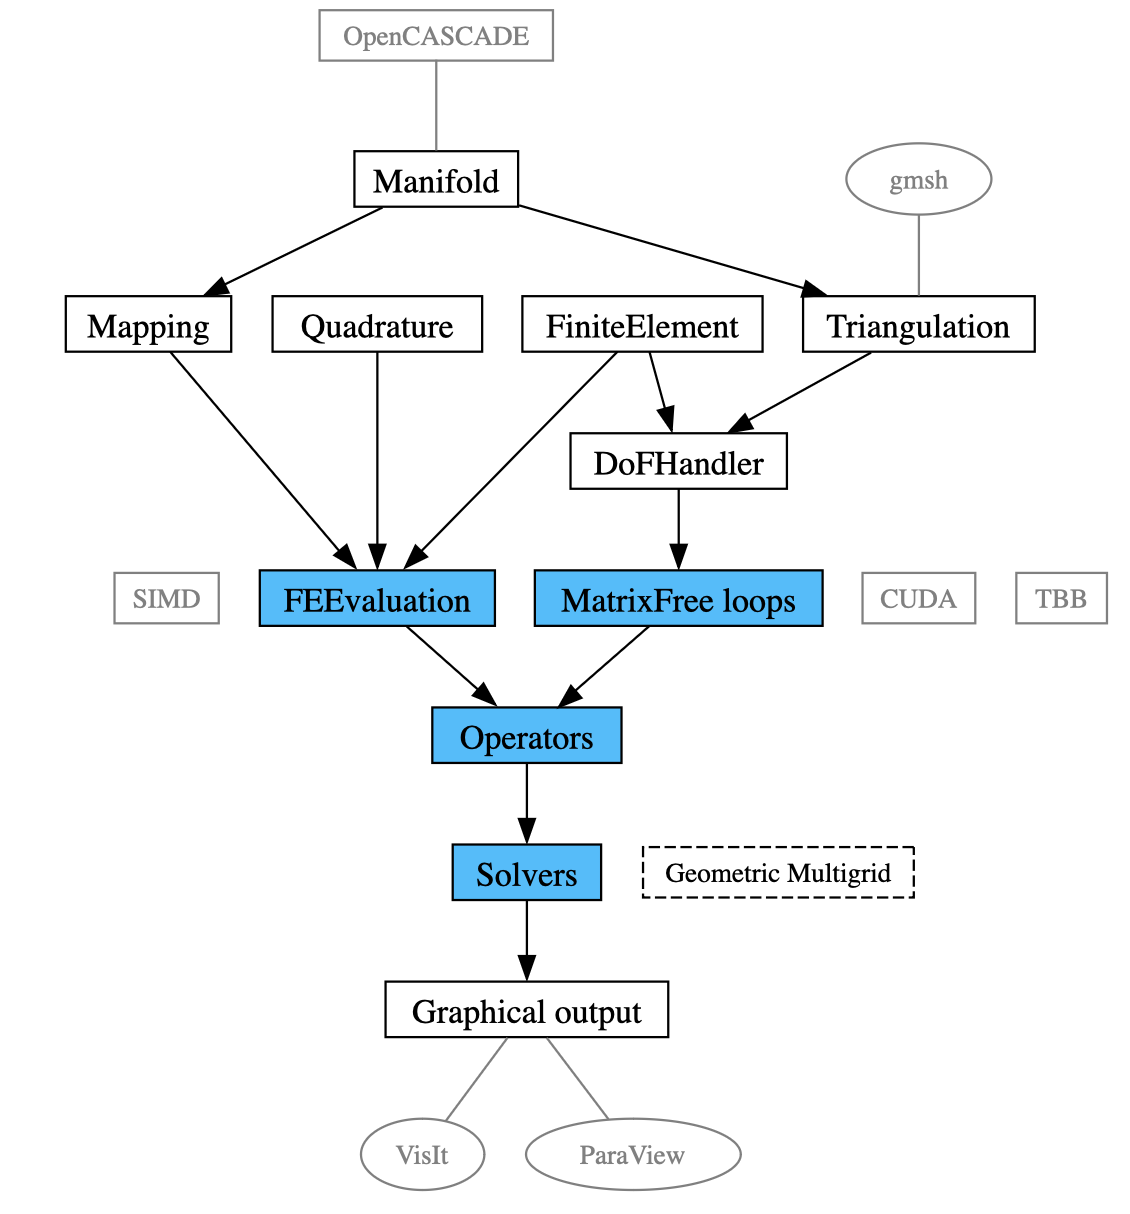
\includegraphics[width=0.5\textwidth]{figure/class_structure.png}
    \caption{Matrix free class structure}
    \label{fig:class_structure}
\end{figure}

\subsubsection{FEEvaluation and FEFaceEvaluation}

The FEEvaluation and FEFaceEvaluation class provides the same functionality as their classical counterpart, FEValues and FEFaceValues, for efficient evaluation and integration of finite element functions on cells and faces respectively. It inherits from FEEvaluationAccess and FEEvaluationBase classes, which handle access to vector data and basic operations, respectively. All these classes are templated on a wide range of arguments such as: dimension, number of components, number type (e.g. double or float), polynomial degree and number of quadrature points per spatial direction, in order to provide enough information on the problem to preform all available compile-time optimizations.

\subsubsection{Matrix Free}


The MatrixFree class itself does not compute or implement any shape function values. Instead, its primary role is to cache and provide efficient access to precomputed data related to shape functions, degree of freedom indices, and geometry mappings, in particular it handles:

\begin{itemize}
    \item \textbf{DoFInfo}: It stores how local degrees of freedom relate to global degrees of freedom.
    \item \textbf{MappingInfo}: It stores the transformations from real to unit cells that are necessary in order to build derivatives of finite element functions and find the location of quadrature weights in physical space.
    \item \textbf{ShapeInfo}: It contains the shape functions of the finite element, evaluated on the unit cell.
\end{itemize}

Apart from these information the only other usage of this class is the implementation of the cell\_loop method, which loops over all the cell in a way that ensures that cells sharing degrees of freedom are not processed concurrently. This property allows for parallel writing without the need for explicit synchronization or locking mechanisms.

\section{Implementation details}
In this section we provide an overview on our implementation focusing on the design decision and on the relevant optimizations we implemented on the code.

The solver we implemented is mainly based on the \verb|deal.II|'s tutorial 37 and 50 for what concerns the matrix-free infrastructure and the parallel matrix-based geometric multigrid used as reference, as well as the \verb|deal.II|'s documentation.

\paragraph{Inhomogeneous Dirichlet BC}
Since the matrix-free infrastructure does not provide any method to algebraically impose non-homogeneous Dirichlet BC, they must be addressed in other ways. In our implementation we employed the lifting technique that, as shown in (\ref{eq:weak}), adds a contribution to the rhs, then solves the same problem with homogeneous Dirichlet BC, and finally sums up the obtained solution to the lifting function.

\paragraph{Geometric Multigrid}
To speed up the convergence of the CG method, our solver implements a geometric multigrid (GMG) technique. The latter is a good fit for a matrix-free algorithm since it can be entirely expressed as matrix-vector products and so its implementation does not require knowledge of the elements of the system matrix (this is not true for other common preconditioners as SSOR or AMG).
In our implementation the GMG leverage the Chebyshev iteration being an effective and easy to parallelize smoother that also fits the matrix-free implementation since it only needs matrix-vector products.

\paragraph{Scalar Type}
In order to reduce the processing time, \verb|float| numbers are used for the multigrid level matrices since they are just a preconditioner and so there is no gain in having more precision and single precision arithmetics is executed in half the time than 
\verb|double| one. The latter is used only for the final matrix since here precision is a concern. This optimization is implemented templating the scalar type used in the ADR matrix-free operator representing the system matrix.

\paragraph{Parallelization} The \verb|MatrixFree| class provides ways to be parallelized on three levels: MPI parallelization on multiple nodes, thread parallelization scheduled by the Threading Building Blocks (TBB) library, and finally with a vectorization by working on a batch of two (or more) cells via SIMD data type (i.e. \verb|VectorizedArray|). We configured this solver to exploit all these levels with MPI across processors, threading on the available physical cores on a processor, and SIMD instructions based on the underlying architecture (e.g., if the AVX512 extension is supported, we can process in parallel 8 \verb|double| operations and 16 \verb|float| operations). Moreover the triangulation is distributed in chunks of roughly equal size across nodes using the \verb|p4est| library.


\section{Results}
In this section we provide our findings about the evaluation of our implementation (\verb|mf|), also comparing it with respect to the matrix-based GMG implementation (\verb|mg|) and to the matrix-based standard implementation (\verb|mb|). The latter just to provide a general idea of the improvements obtained from the parallel implementation we saw during the course, meaning that it should not be considered in the actual comparison study between matrix-free and matrix-based solvers.

It is important to note that our rigorous comparison is based on two solvers that differs only on the \verb|deal.II| matrix implementation, i.e. matrix-free or matrix-based, that now on may be referred as \verb|mf| and \verb|mg| respectively, while the previously mentioned simple solver may be referred as \verb|mb|. Where \verb|mg| stays for multigrid, just to differentiate it from the \verb|mb| simple implementation. Moreover, the \verb|mb| implementation is provided with smaller problem size since it cannot handle huge problems as the other multigrid solvers.

The tests have been submitted to the \verb|gigatlong| queue in the MOX cluster at Politecnico di Milano.

One last remark, during the evaluation of our matrix-free implementation, multi-threading has been disabled for two main reasons: firstly to be consistent to the other reference implementations, lastly to exploit as much the computational resources of the used node spawning a process for each physical core.


\subsection{Convergence}
The convergence study for our matrix-free solver is run with finite elements having polynomial degree 2 and the known solution for the previously constructed problem is in \(L^\infty\), so we expect a quadratic convergence for the \(L^2\) error and a cubic convergence for the \(H^1\) error accordingly. The resulting convergence table is reported in Table (\ref{tab:conv_mf}) proving our assumptions. 

\begin{table}[h]
    \centering
    \begin{tabular}{|c|c|c|c|c|}
        \hline
        Cells & L2 error & L2 order & H1 error & H1 order \\
        \hline
        1024 & 2.330877e-06 & -  & 4.834520e-04 & - \\
        4096 & 2.913946e-07 & 3.00 & 1.208651e-04 & 2.00 \\
        16384 & 3.642542e-08 & 3.00 & 3.021641e-05 & 2.00 \\
        65536 & 4.553212e-09 & 3.00 & 7.554112e-06 & 2.00 \\
        \hline
    \end{tabular}
    \caption{Convergence table for our matrix-free implementation solving the above problem with finite element polynomial degree 2.}
    \label{tab:conv_mf}
\end{table}


\subsection{Time complexity}

The Table (\ref{tab:dim_time}) provides a comparison of setup + assemble and solve times between the Multigrid Matrix-based and Matrix-free implementations as the number of Dofs increases. This table clearly shows that the matrix-free implementation is faster than the matrix-based one and keeps improving performances as the number of Dofs increases. In particular the \verb|mf| starts from being more than three times as fast for the solver, and more than two times as fast when it comes to initialization costs, until reaching, for the maximum number of Dofs, more than 6 time of speedup for the solver and 4 for the setup+assemble. Considering instead the total time of execution, the matrix free starts form a 2 times speedup and is able to reach a 5 times speedup with the maximum number of Dofs.\\
 In particular, it's evident that the main deviation between the two methods occurs between 4096 and 16384 Dofs, when probably the cache in the processor can no longer hold all data necessary for the matrix-vector products and all matrix elements must be fetched from main memory, causing a decay of the \verb|mb|'s performances.

\begin{table}[h]
    \centering
    \begin{tabular}{|c|c|c|c|c|}
        \hline
        & \multicolumn{2}{c|}{Multigrid Matrix-based} & \multicolumn{2}{c|}{Matrix-free} \\
        \cline{2-5}
        n\_dofs & Setup+assemble & Solve & Setup+assemble & Solve \\
        \hline
        263169 & 0.0857816 & 0.128677 & 0.0472224 & 0.0425927 \\
        1050625 & 0.289255 & 0.441476 & 0.114377 & 0.137391 \\
        4198401 & 1.18131 & 2.04448 & 0.367881 & 0.359345 \\
        16785409 & 4.71038 & 9.84222 & 1.29147 & 1.33877 \\
        67125249 & 19.0633 & 33.6557 & 4.82622 & 5.47594 \\
        \hline
    \end{tabular}
    \caption{Table comparing setup + assemble and solve time needed by our mg and mf implementations as the number of Dofs increases}
    \label{tab:dim_time}
\end{table}


The plot in Figure (\ref{fig:time_dim}), instead, shows the same relation as before between execution time of the problem and an increase of its size, but considering the execution of each method with a different number of processes, form 8 to 32.
It's evident that for all the solvers as the number of Dofs increases, the best performances are obtained with the largest number of processes.
Though, it's interesting to see how \verb|mf| and \verb|mg| shows a linear behaviour in the time needed for the execution, while the \verb|mb| shows a quadratic one.  This probably depends on the fact that the \verb|mb| has to perform a number of iterations which depends on the size of the problem.
\begin{figure}[h]
    \centering
    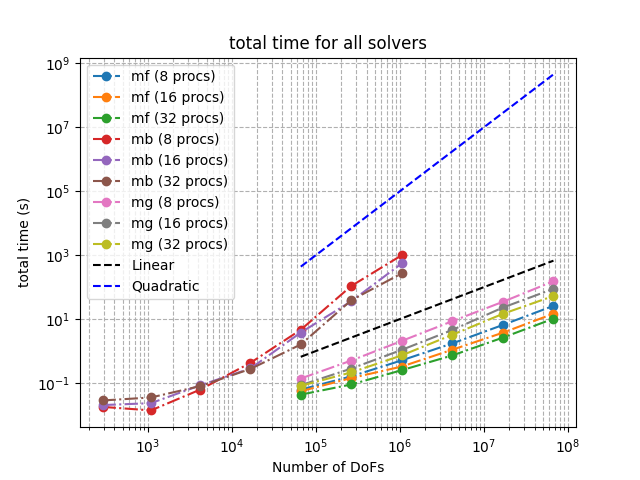
\includegraphics[width=0.8\textwidth]{figure/time_total.png}

    \caption{Total execution time plot over increasing number of Dofs comparison between all the solvers with respectively 8, 16 and 32 processes each one}
    \label{fig:time_dim}
\end{figure}


\subsection{Scalability}
In order to compare how the matrixfree and matrixbased implementations scale, timing data has been collected varying the number of processes and the problem size. Scaling experiments have been performed on Q2 elements, solving the previously defined problem in 2D.

A comparison between all the three solvers is provided in Figure (\ref{fig:strongcomp}) while a focus on the matrixfree (\verb|mf|) and matrixbased multigrid (\verb|mg|) solvers is provided in Figure (\ref{fig:strong_mg_mf}).
Along the lines, the problem size is held constant as the number of cores is increasing. When doubling the number of cores, one expects a halving of the computational time, indicated by the black dashed ideal scaling lines. The above mentioned behaviour is referred as strong scaling.
\begin{figure}[h!]
     \centering
     \begin{subfigure}[h]{0.7\textwidth}
         \centering
         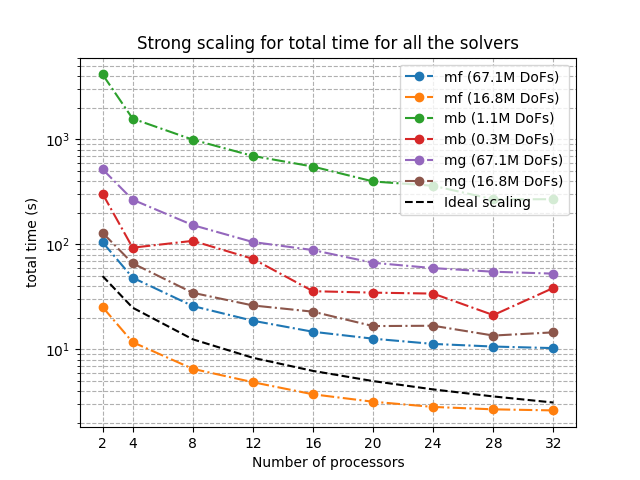
\includegraphics[width=\textwidth]{figure/strongcomp_total.png}
         \caption{Total time}
     \end{subfigure}
     \begin{subfigure}[h]{0.5\textwidth}
         \centering
         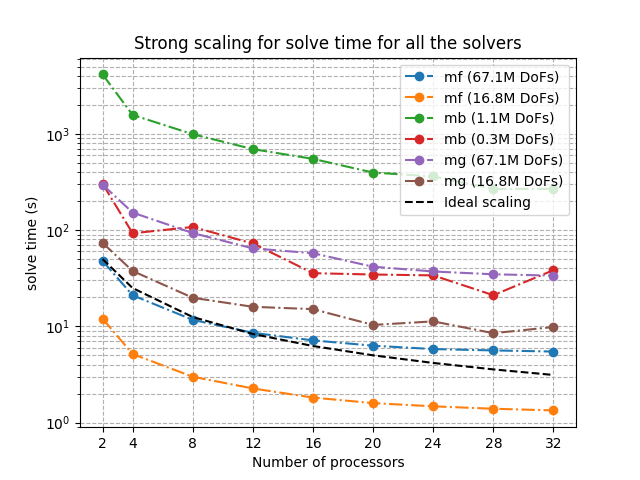
\includegraphics[width=\textwidth]{figure/strongcomp_solve.png}
         \caption{Solve time}
     \end{subfigure}
     \hspace*{-0.4cm}
     \begin{subfigure}[h]{0.5\textwidth}
         \centering
         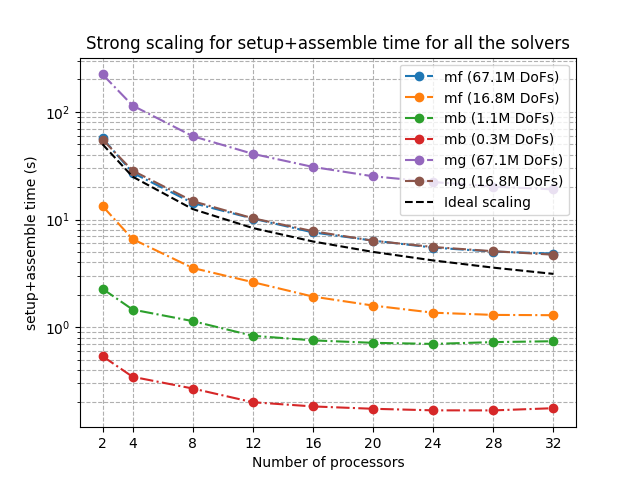
\includegraphics[width=\textwidth]{figure/strongcomp_setup+assemble.png}
         \caption{Setup and assemble time}
     \end{subfigure}
     \caption{Total, solve, and setup+assemble time scaling comparison between all the solvers for the two highest problem sizes. Strong scaling can be compared with the reference lines, weak scaling can be assessed knowing that each plot differs quadruplicates the problem size.}
     \label{fig:strongcomp}
\end{figure}

Figure (\ref{fig:strongcomp}) shows that the \verb|mf| and \verb|mg| solvers follow a similar behaviour for all the considered times. They show an almost ideal behavior for the strong scaling until around 12 to 16 processors, then the curve start flattering. This behaviour may be caused by the overhead being slightly higher for inter-CPU communications than for intra-CPU ones.

Moreover setup and solve time is a bit suboptimal starting from fewer processors than the solve one. The latter starts to show a suboptimal behaviour around 12 to 16 processors, so it is the one that produces this behaviour on the total time.

Lastly, considering the basic matrixbased implementation (\verb|mb|), it is possible to see a quite unstable behaviour while scaling, being also influenced by fluctuations on \textbf{iteration count}. This tells us that it is not a good choice for exploiting huge parallelism. Both multigrid solvers have a very stable behaviour also regarding the iteration count that is almost constant around 6 iterations in all the studied conditions, making possible to solve very large problems with few iterations.
\begin{figure}[h]
     \centering
     \begin{subfigure}[h]{0.5\textwidth}
         \centering
         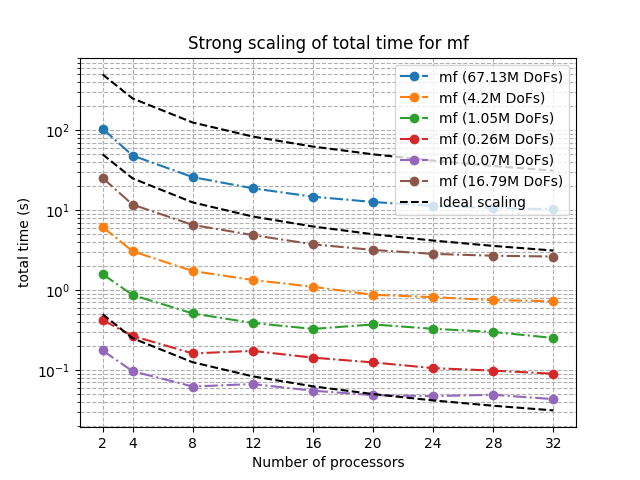
\includegraphics[width=\textwidth]{figure/strong_mf_total.png}
         \caption{Matrixfree}
     \end{subfigure}
     \hspace*{-0.4cm}
     \begin{subfigure}[h]{0.5\textwidth}
         \centering
         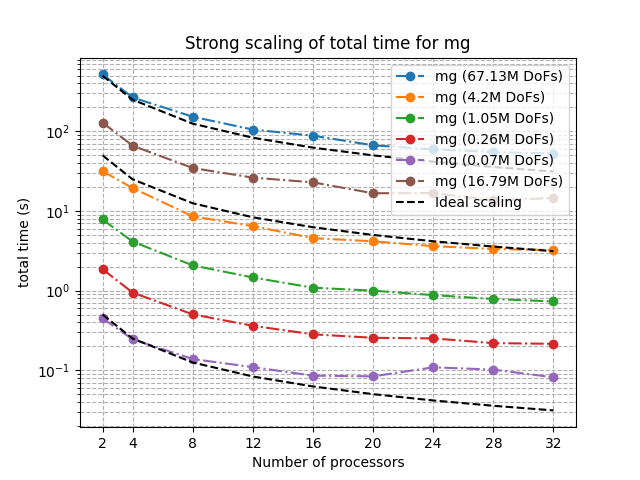
\includegraphics[width=\textwidth]{figure/strong_mg_total.png}
         \caption{Matrixbased}
     \end{subfigure}
     \caption{Total time scaling for both matrixfree and matrixbased multigrid solvers. Strong scaling can be compared with the reference lines, weak scaling can be assessed knowing that each plot differs quadruplicates the problem size.}
     \label{fig:strong_mg_mf}
\end{figure}


Considering now Figure (\ref{fig:strong_mg_mf}),  it is possible to see that both \verb|mf| and \verb|mg| solvers have a good strong scaling larger problems (i.e. above few M Dofs), while they perform not so good with smaller ones. The \verb|mg| implementation shows a slightly better strong scaling than the \verb|mf| one, but the latter solves a problem 4 times bigger in the same time.

From Figure (\ref{fig:strong_mg_mf}) it is also possible to evaluate the \textbf{weak scaling} behaviour, just considering that each line differs by a factor 4 in the number of Dofs, and that an ideal weak scaling is obtained when doubling both the number of Dofs and the number of processors gives the same total time. Given this definition, weak scaling is optimal for few processors (i.e. from 2 to 8, and from 4 to 16) and smaller problem sizes for both solvers. While for higher count of processors and problem sizes it becomes suboptimal.

In summary matrixfree implementation shows similar scaling behaviour that the matrixbased one, considering almost same underlying implementation (obviously, except for the matrix representation) and problem to solve. Analysing this data it is worth noting that our hardware resources are quite limited and more clear scaling data should be collected on hundreds of processes, doubling their count at each run.


\subsection{Polynomial degree efficiency}
In order to evaluate the actual efficiency of the matrixfree (\verb|mf|) solver with respect to the matrixbased (\verb|mg|) one at different polynomial degrees, it is possible to look at the throughput of the 2D multigrid solvers at different values for the finite element polynomial degree.

To do so, timing data has been collected for problems around 10M Dofs, varying only the polynomial degree, then the MDofs/s metric has been computed for both solve and setup+assemble phases.
\begin{figure}[h!]
     \centering
     \begin{subfigure}[h]{0.5\textwidth}
         \centering
         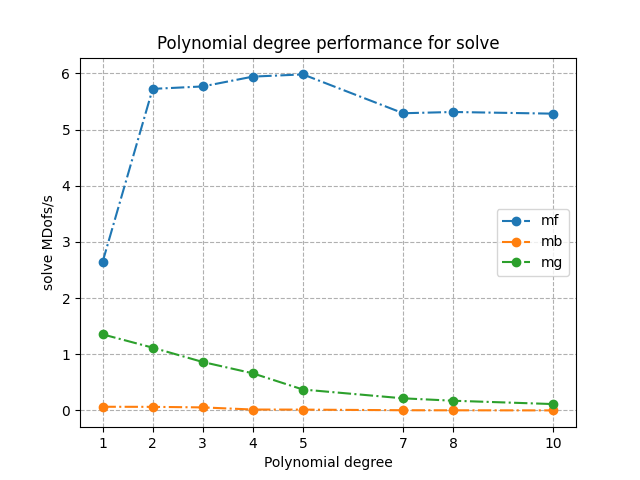
\includegraphics[width=\textwidth]{figure/polynomial_solve.png}
         \caption{Solve}
     \end{subfigure}
     \hspace*{-0.4cm}
     \begin{subfigure}[h]{0.5\textwidth}
         \centering
         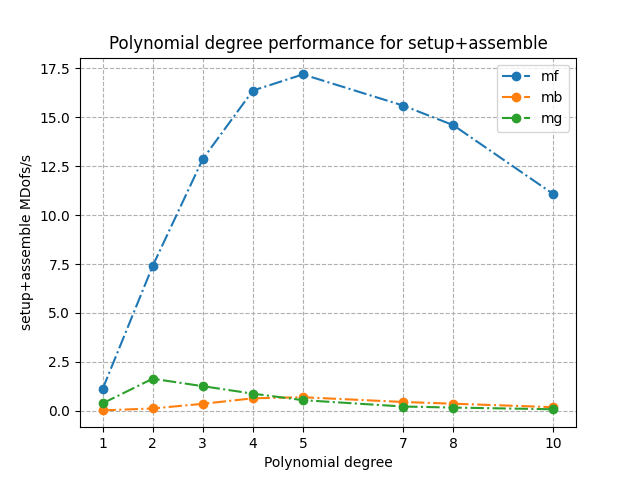
\includegraphics[width=\textwidth]{figure/polynomial_setup+assemble.png}
         \caption{Setup + assemble}
     \end{subfigure}
     \caption{Comparison of the solvers based on processed MDoFs per second in both solve (a) and setup+assemble (b) at different polynomial degrees.}
     \label{fig:poly}
\end{figure}
From Figure (\ref{fig:poly}) it is firstly possible to note that while both matrixbased implementations have very poor throughput, the matrixfree one provides a \(6\times\) gain in solve time.

A more clever point is related to the actual shape of the curves. The matrixfree solver shows a throughput peak around a 4-5 polynomial degree for both the phases. \verb|mf| solve time is less affected, except for degree 1, while setup time is more sensible to the polynomial degree.
On the other hand, solve throughput for the matrixbased multigrid solver is decreasing as the degree increases, while its setup throughput has a slight peak in 2.

Summing up, the matrixbased implementation is mostly effective when solving problems with polynomial degree around 5. So switching from a matrixbased implementation to a matrixfree one it is possible to get more precise results (provided a sufficiently smooth solution) in a shorter time.

\subsection{Time speedup}
To evaluate in a more formal way the actual time speedup of our matrixfree implementation (\verb|mf|) with respect to the multigrid matrixbased one (\verb|mg|) it is possible to plot the ratio between their solve time as function of the problem size. For all the evaluated processors count, it follows a logarithmic speedup up to a problem size of 10M Dofs, then it suffers a bit for the runs with an higher number of processors. This can be due to the communication overhead among CPUs that bounds the faster matrixfree implementation, while for the matrixbased one the bound is imposed by the memory access.

\begin{figure}[h]
    \centering
    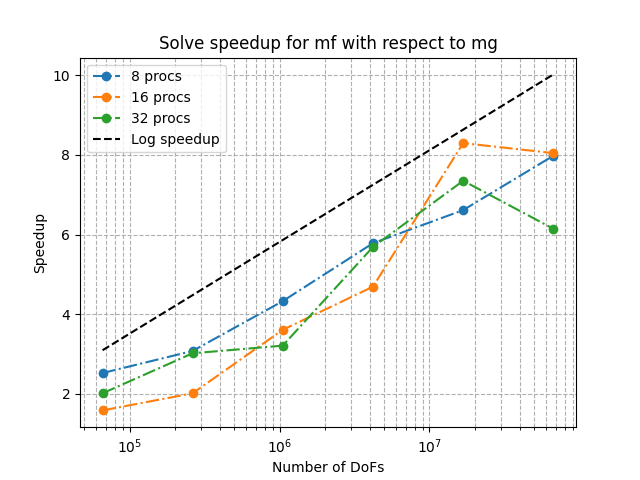
\includegraphics[width=0.8\textwidth]{figure/speedup_mf_mg.png}

    \caption{Total execution time plot over increasing number of Dofs comparison between all the solvers with respectively 8, 16 and 32 processes each one}
    \label{fig:speedup}
\end{figure}


\subsection{Memory efficiency}
To evaluate the improvement in memory occupation that the matrixfree implementation provides with respect to the matrixbased one, one possibility is to profile the heap occupation and compare the memory footprint of both solvers.

In Figure (\ref{fig:mem_foot}) provides the graphical representation of the Valgrind's massif heap profiler output. Both solvers are run with the same problem with 1M Dofs in order to compare the memory usage.

The plots shows that the matrixfree solver have a peak that is approximately one half of the matrixbased one, meaning that in the same hardware can fit a problem that is double in size. Specifically, for a 1M Dofs problem, the matrixfree have a peak of 540 MiB with an average level of 500 MiB during the evecution. On the other hand the matrixbased one demands for an increasing memory occupation till reaching a peak of 931 MiB.

In the matrixfree solver the most of the memory demand is for the storage of the evaluated coefficients that must be aligned in memory to leverage the \verb|deal.II| vectorization and so occupying more space, and for the storage of the rhs vector.
On the other hand, as one can guess, the matrixbased solver occupies most of the memory with the storage of the matrix.

\begin{figure}[h!]
     \centering
     \begin{subfigure}[h]{0.47\textwidth}
         \centering
         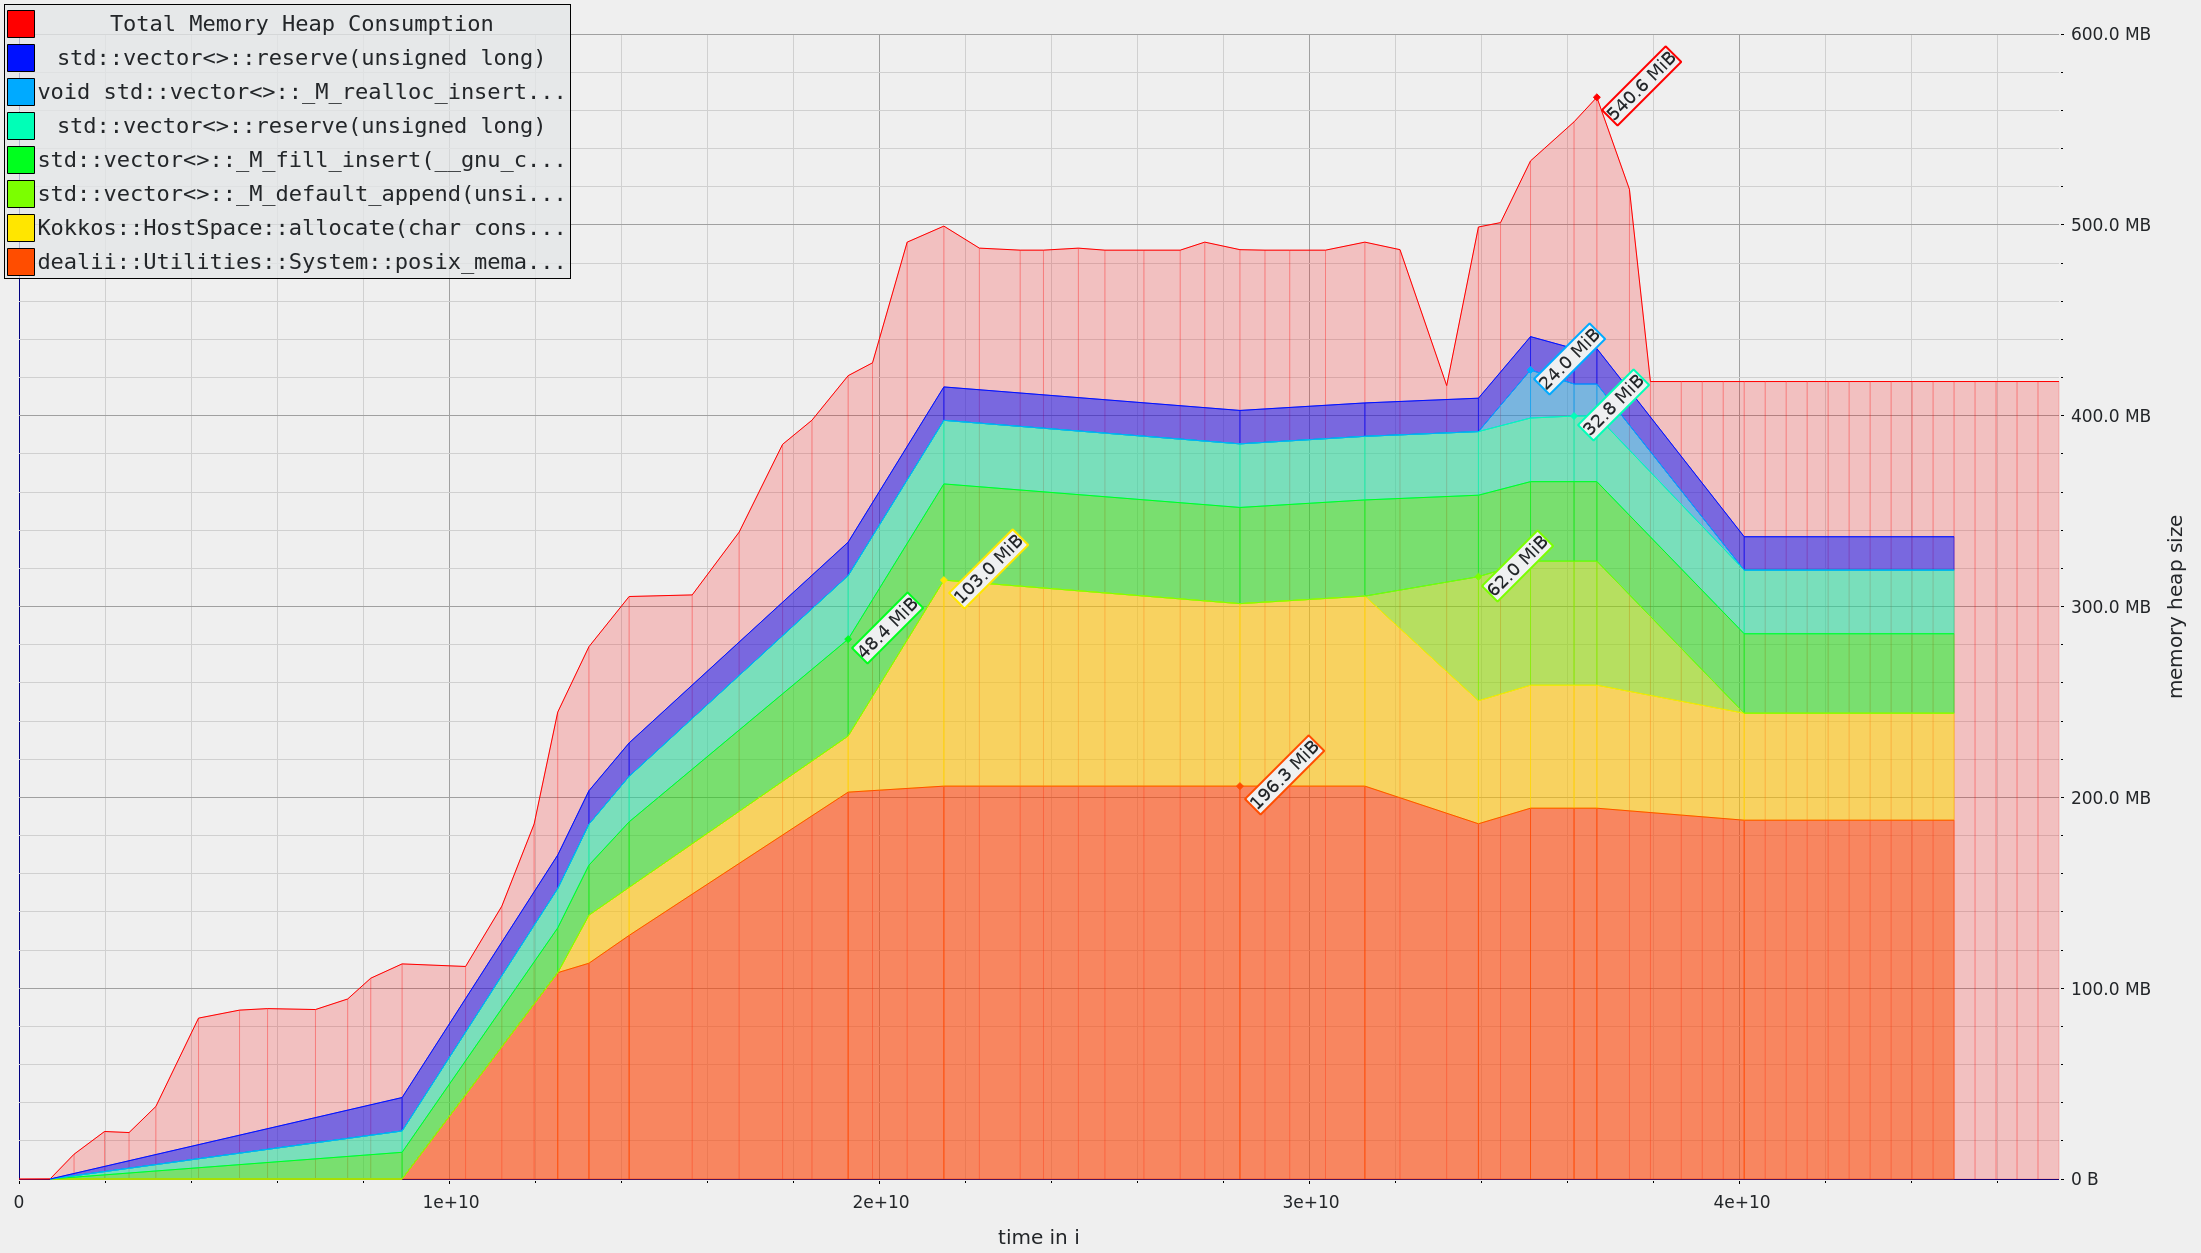
\includegraphics[width=\textwidth]{figure/massif-mf.png}
         \caption{Matrixfree}
     \end{subfigure}
     \hspace*{-0.2cm}
     \begin{subfigure}[h]{0.47\textwidth}
         \centering
         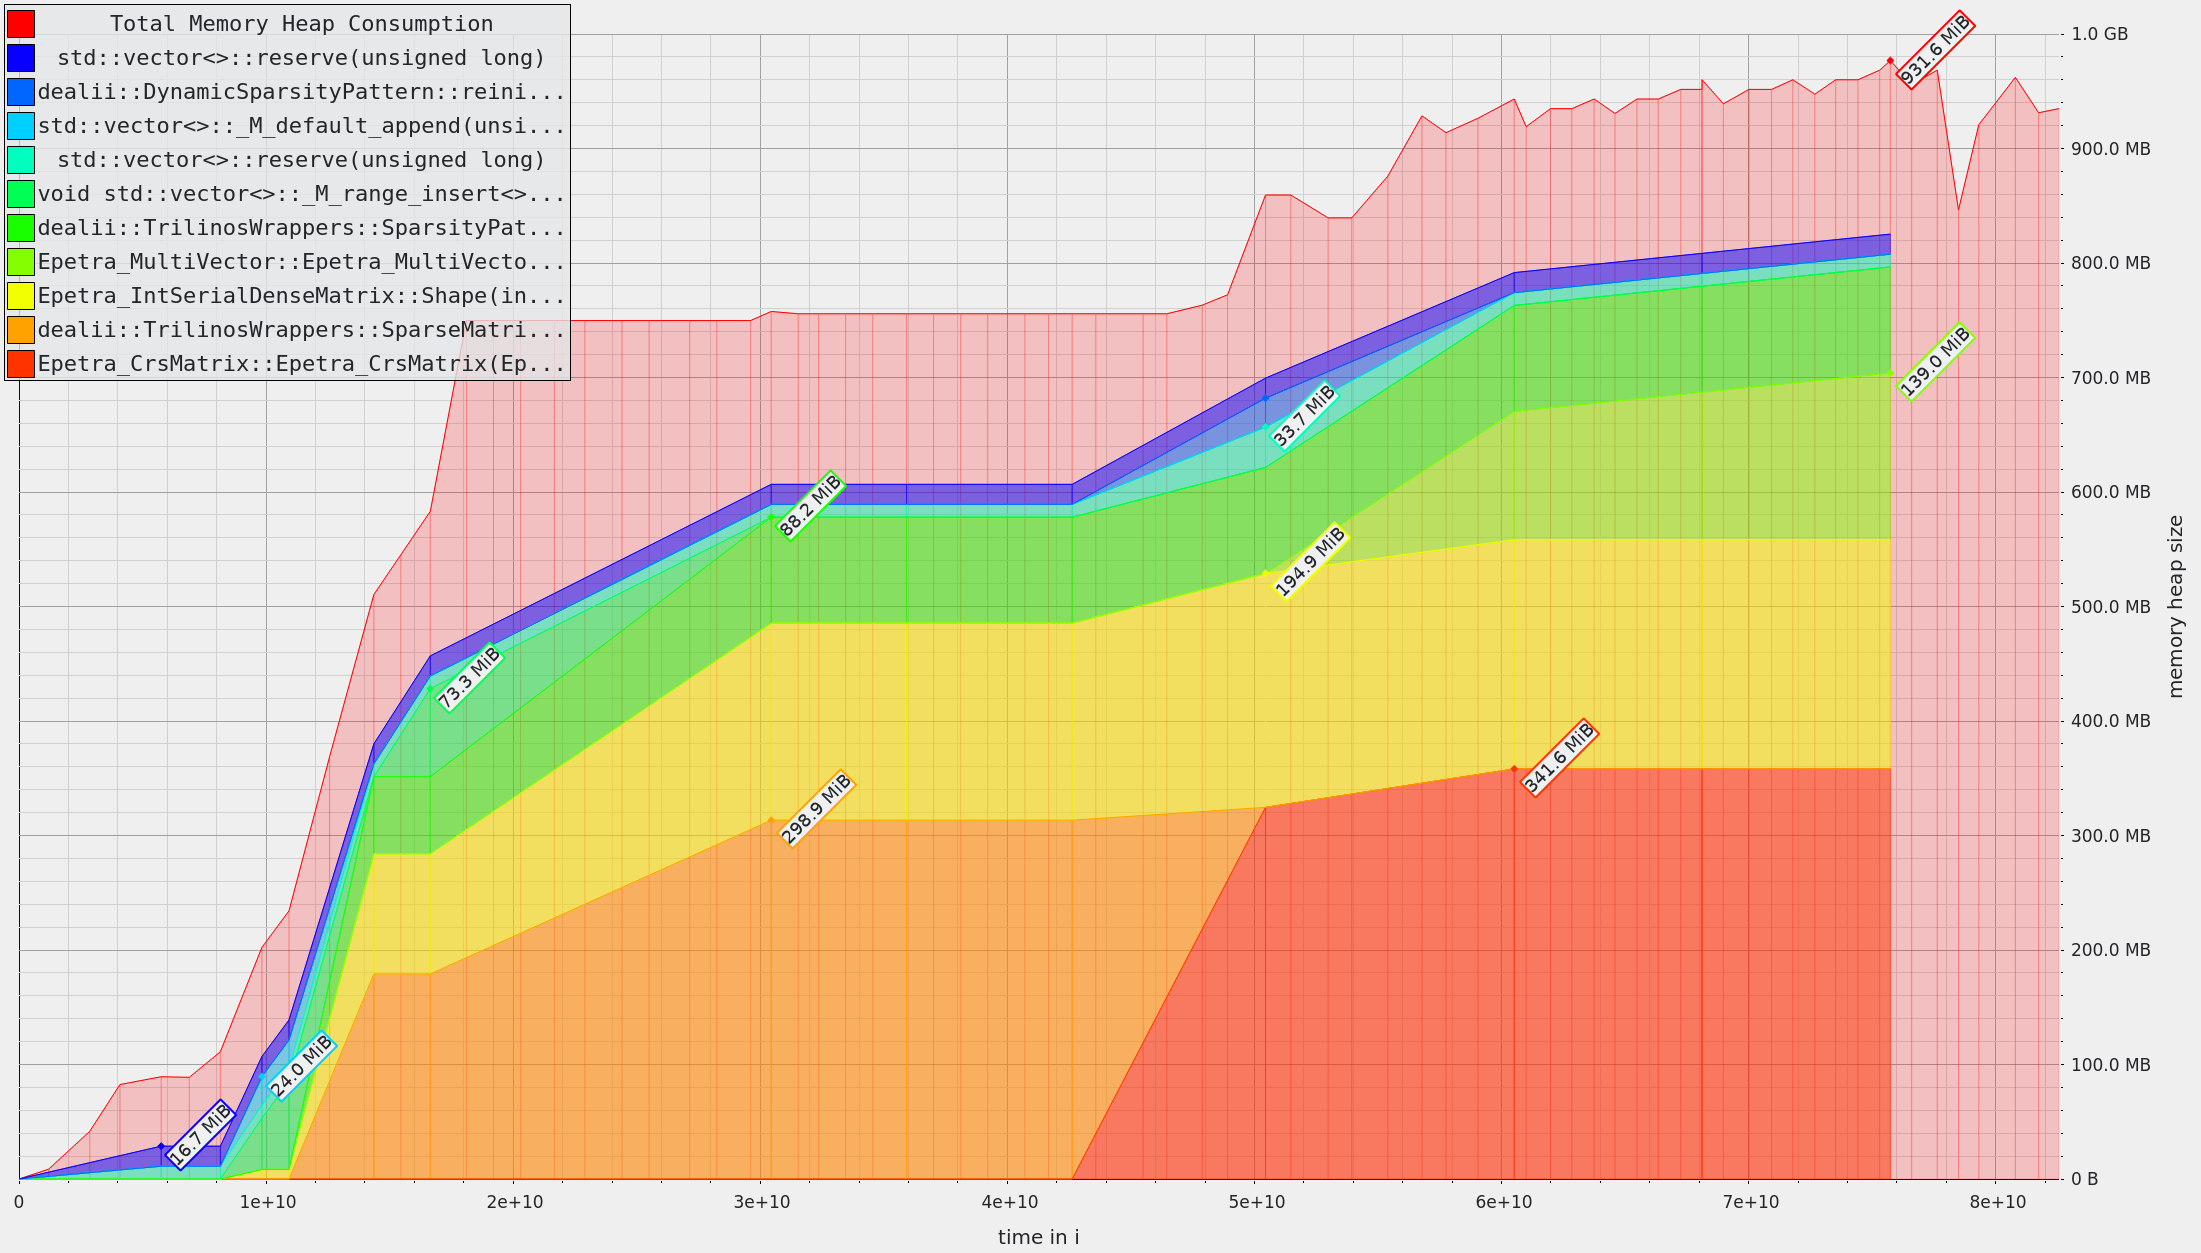
\includegraphics[width=\textwidth]{figure/massif-mg.png}
         \caption{Matrixbased}
     \end{subfigure}
     \caption{Heap memory footprint for the solution of the problem with 1M Dofs.}
     \label{fig:mem_foot}
\end{figure}



\subsection{Implementation complexity}
The implementation of the matrixfree problem has been based, as previously said, on the Deal.II infrastructure. This means we have had to consult extensively deal.II documentation as well as its tutorial steps.
Undoubtedly, one of the main difficulties, lied in the fact that the matrixfree implementation of the solver asks for a complete re-elaboration of the mindset in the way in which the problem resolution has to be performed. In fact, the presence of a class that reflects the Matrix behaviour, although the matrix is never effectively assembled, means that problems such as the efficient application of boundary conditions and the handling of coefficient functions have to be addressed in a different way with respect to what is done for the matrix-based approach. In fact, for example, not having a matrix to modify, constraints have to be enforced during the matrix-vector product computations, adjusting vector entries directly to respect the boundary conditions. Instead, for what concern coefficients functions, these are no more evaluated on the fly, but are precomputed and stored in appropriate data structure, which allows efficient access during matrix-vector product computations without repeatedly evaluating the functions.

Moreover since the matrix free implementation is intrinsically more computationally expensive a great deal of care has to be put into reorganizing the data in efficient structures and scheduling them accordingly. Part of this effort is done by the library itself (like for the cell\_loop method) as well as imposing a vectorized specialization of all the methods involved in the computation. 

Obviously the automatic scheduling means that the loop is not as clear as the classical approach and leaves the developer with less flexibility in applying their problem-specific restrictions, however some of these limitations have been lifted by the recent addition of more, but still limited, function capabilities; still, the underlying problem persists.

While these constraints allow for a guaranteed efficiency of the implementation, they put a significant burden on the developer which has to reinterpret the problem in an unusual way, closer to the hardware than to the mathematical problem itself.

\printbibliography % Print the bibliography

\end{document}